\documentclass[a4paper,11pt]{jsarticle}


% 数式
\usepackage{amsmath,amsfonts}
\usepackage{bm}
\usepackage{physics}
% 画像
\usepackage[dvipdfmx]{graphicx}
% ローマ数字
\usepackage{otf}
% 単位
\usepackage{siunitx}
% 表
\usepackage{multirow}
% 化学反応
\usepackage[version=4]{mhchem}

\begin{document}

\title{理論演習 プログラムの修正からゴミ分子の導入まで}
\author{齋藤駿一}
\date{\today 編集}
\maketitle

\section{概要}
まず,前回考えた微分方程式の変数から体積を除き,栄養分子から膜分子までのパスが存在しないとき反応ネットワークを作り直すようにプログラムを修正した.
その結果,$p$が小さいとき濃度が発散する成分が見られたので,それについて考察した.

次に,姫岡先生のモデルを参考にしてゴミ分子を導入した.
ただし,ゴミ分子以外の成分が発散した場合に反応ネットワークを作り直すようにプログラムを修正した.
このプログラムを実行し,栄養成分と成長率の関係をプロットした.

\section{プログラムの修正}
まず,今回は栄養分子は1種類のみと仮定した.
概要で述べた修正を行い,成分数を$N=5$,connection rateを$p=0.1$,栄養濃度を$n=1$,酵素反応の反応速度をどれも$1$として,時刻$T=1000$まで計算を行った.
その結果,全成分濃度が定常に至ることもあれば,図\ref{fig:nonwaste_cons_div_N5_2}のように,ある成分が発散することもあった.

これは,栄養分子から膜分子への自己触媒反応が存在しない,または膜分子の自己触媒よりも素早く増殖する成分があることを示唆している.
そこで,この図のような計算結果をもたらす反応ネットワークを確認した.
その結果,やはり膜分子の自己触媒ができていないケースもあったが,その一方で,膜分子の自己触媒サイクルは存在しているにもかかわらず成長率が$5\times 10^{-3}$程度と低く,発散する成分が見られるような場合もあった(これは板書する).


\begin{figure}[htbp]
  \centering
  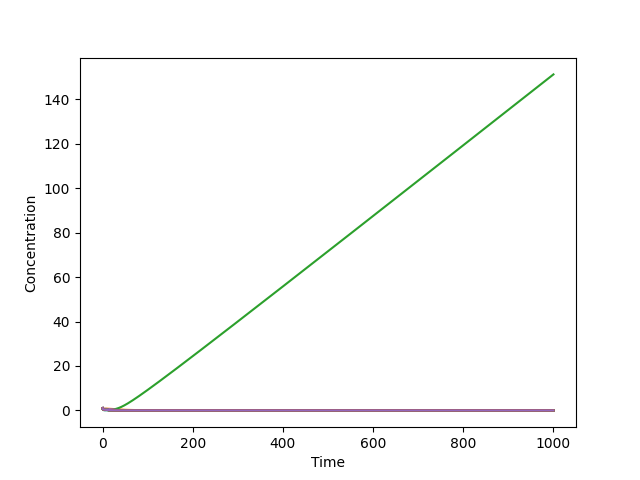
\includegraphics[width=10cm]{nonwaste_cons_div_N5_2.png}
  \caption{濃度が発散する例.膜分子などの成分の濃度は紫色の線に重なっており,緑色の線で表されるある成分の濃度が定常になっていない.}
  \label{fig:nonwaste_cons_div_N5_2}
\end{figure}

\section{ゴミ分子の導入}
次に,これまで考えてきた(活性のある)成分$\ce{P_i}\,(i=0,1,\cdots,N-1)$のそれぞれに対して,(活性のない)ゴミ分子$\ce{W_j}\,(j=0,1,\cdots,N-1)$の存在を仮定した.
こうしたゴミ分子$\ce{W_j}$は,酵素反応$\ce{P_i + P_k -> P_j + P_k}$がある確率$\epsilon$で失敗し,$\ce{P_i + P_k -> W_j + P_k}$が起こってしまうことで生成すると考えた.
さらに,活性のある成分$\ce{P_i}$とゴミ分子$\ce{W_j}$が反応速度$k_p$で結合して複合体$\ce{C_{ij}}$を作るとした.
また,複合体形成の逆反応も反応速度$k_m$で起こるとした.

また,先ほどのようにある成分濃度が発散するような反応ネットワークを避けることにした.
具体的には,最終時刻$t=T$での(活性のある)成分$i=0,\cdots,N-1$の濃度$[\ce{P_i}](t)$の時間変化率
\begin{equation}
  \frac{[\ce{P_i}](T)-[\ce{P_i}](T-dt)}{dt}
\end{equation}
の2乗和が$10^{-8}$を超えた場合,反応ネットワークを作り直すようにした\footnote{この閾値は経験的に決めた.}.

以上の仮定の下で,$N=5,p=0.8,\epsilon=0.001,k_p=0.1,k_m=0.001$とし,$n=10^{-5},10^{-4},10^{-3},10^{-2},10^{-1},1,10,10^2$のそれぞれに対して5通りのランダム反応ネットワークを作り,それらの最終的な($t=T$での)成長速度の平均値$\mu$を計算した.
その結果,$n$に対する成長速度$\mu$の関係は,図\ref{fig:waste_10n}のようになった.
この結果は,$N=10$に変更しても変わらなかった(図\ref{fig:waste_N10_p08}).

\begin{figure}[htbp]
  \centering
  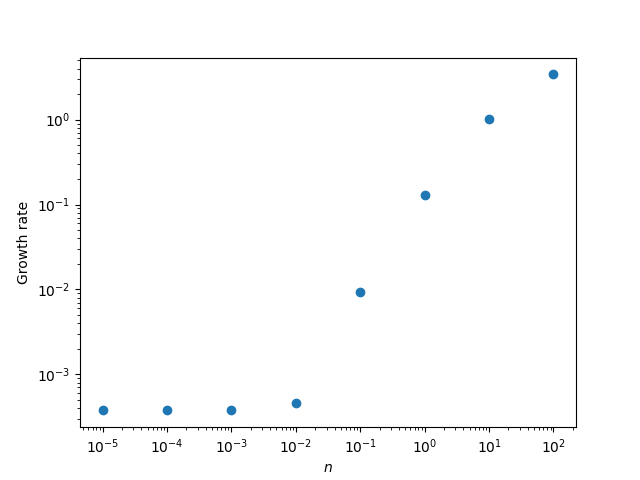
\includegraphics[width=10cm]{waste_10n.png}
  \caption{$N=5$での栄養濃度と成長速度の関係.$n=10^{-2}$と$n=10^{-1}$の間で成長率の振る舞いが大きく異なる.}
  \label{fig:waste_10n}
\end{figure}

\begin{figure}[htbp]
  \centering
  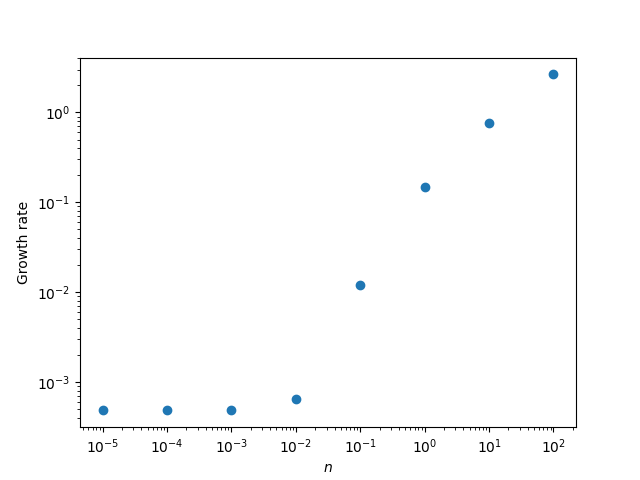
\includegraphics[width=10cm]{waste_N10_p08.png}
  \caption{$N=10$での栄養濃度と成長速度の関係.}
  \label{fig:waste_N10_p08}
\end{figure}

\end{document}